\documentclass[11pt]{article}

% "review" = anonymous submission version. Change to "final" for camera-ready.
\usepackage[review]{acl}

\usepackage{times}
\usepackage{latexsym}
\usepackage[T1]{fontenc}
\usepackage[utf8]{inputenc}
\usepackage{microtype}
\usepackage{inconsolata}
\usepackage{graphicx}
\usepackage{booktabs}
\usepackage{amsmath}

\newcommand{\cond}[1]{\texttt{#1}}

\title{No critical period in language-model pretraining:\\
       the later deficit is the one repaired more slowly}

\author{Anonymous ACL submission}

\begin{document}
\maketitle

\begin{abstract}
Vision networks have critical periods: a stimulus deficit applied during an
early window of training permanently reduces final accuracy, however long the
network is afterwards trained on clean data. We test the analogous claim in
autoregressive language-model pretraining. Because a loss difference at a
single training budget cannot distinguish permanent damage from recovery that
has not finished, we measure the \emph{rate} at which damage is repaired: the
same conditions are trained at a ladder of budgets and the gap to a
seed-matched clean baseline is fitted as $\mathrm{gap}(T) = c/T^{\alpha}$. The
exponent is read against a negative control measured in the same experiment,
never against a theoretical value. At 7.34M parameters on TinyStories, across
four budget rungs and eight seeds, a window-shuffle deficit applied at the very
start of training is repaired at the same rate as an information-preserving
control of identical size and onset ($\Delta\alpha = -0.003$, $p = 0.95$); the
same deficit applied at mid-training is not ($\Delta\alpha = -0.395$,
$p = 0.0002$). The registered contrast was one-sided in the critical-period
direction and came out the other way. We report two registered results, not
one: an earlier registered run measured the same effect and returned
\cond{INCONCLUSIVE}, and is reported here in full with its cause diagnosed.
\end{abstract}

\section{Introduction}

\citet{achille2019critical} showed that convolutional networks have critical
periods: blur the training images during an early window and final accuracy is
permanently reduced, no matter how long the network is subsequently trained on
clean data, while a deficit that leaves low-level image statistics intact---a
vertical flip---leaves no permanent trace. The effect depends on \emph{when} the
deficit occurred, not only on how much of it there was. It arises in deep linear
networks too \citep{kleinman2024critical}, so it is not an accident of one
architecture.

Does anything like this happen in language-model pretraining? The closest
existing evidence points away from it. \citet{constantinescu2025investigating}
varied the age of exposure to a second language and found \emph{no} critical
period; they had to insert a plasticity-decreasing regularizer to manufacture
one. Their manipulation is delayed exposure to new material rather than degraded
input during a window followed by clean input, so it does not answer the question
directly, but it sets the prior.

We ran the deficit-window protocol itself, and hit a measurement problem that
turns out to be the substance of the paper.

\subsection{A level at one budget cannot answer this}

The natural endpoint is the held-out loss gap at the end of training. It does not
work, and the reason is not subtle: a deficit condition that is merely
\emph{behind}---still closing the gap, just slower---produces the same final gap
as one that is permanently damaged. In our own exploratory runs the gap fell 42\%
on a single budget doubling, so the endpoint was scoring where the run happened
to stop.

Worse, the obvious fix makes it invisible. Annealing the learning rate to zero at
the end of training makes every run converge, which is what one wants for
comparability---and it also freezes in place any condition that had not finished
recovering. Under that schedule a single-budget endpoint reports ``permanent'' by
construction. So we measure the rate instead.

\subsection{What we measure}

Each condition is trained at four budgets, each double the last. The gap to a
seed-matched clean baseline is fitted per seed as $\mathrm{gap}(T) = c/T^{\alpha}$,
and $\alpha$---how fast the damage is repaired as the budget grows---is the
registered quantity.

\textbf{$\alpha$ is read against the negative control, never against a
theoretical value.} The tidy derivation that a pure lag gives $\alpha = 1$
assumes the baseline learning curve's log-slope is constant. Ours falls about
30\% per doubling, so that anchor is wrong, and the value corrected for the
measured slopes is too fragile to replace it. The slope factor is common to every
condition at a rung, so it cancels in a comparison and cancels nowhere else.

This buys a comparative answer and gives up an absolute one. \textbf{Whether the
damage is permanent or merely slow to repair is out of scope}, and
Section~\ref{sec:notshow} says why.

\section{Method}

\subsection{Model and corpus}

A 7.34M-parameter decoder-only transformer (8 layers, $d=256$, 8 heads, context
256, RoPE, tied embeddings) trained from scratch on a 629\,MB prefix of
TinyStories \citep{eldan2023tinystories}---158M tokens under a 4096-entry
byte-level BPE fit on the training text only. The held-out split is the dataset's
own validation file, never subjected to a deficit and never used for any
selection decision. Training runs on a laptop-class accelerator at
32.5k tokens/s.

Learning rate: linear warmup over 2\% of the run, then cosine decay to exactly
zero. The schedule is a registered constant and a named scope limit---%
\citet{pawlak2025occurence} reports that critical-period effects in vision can be
removed by a cyclic schedule, so any result here is conditional on this one.

\subsection{The two deficits}

Both are applied to the training stream only.

\textbf{Deficit S.} Within each non-overlapping window of 16 tokens, permute the
order, resampled for every window of every batch. This destroys local sequential
structure while leaving every sequence a permutation of itself.

\textbf{Deficit F (negative control).} The \emph{same} operation with a single
permutation drawn once for the whole study and reused everywhere. The reordering
is therefore deterministic and invertible: nothing is destroyed, and a model can
in principle learn to read the scrambled order.

Same operation, same locus, same surface magnitude, differing in exactly one
property. That is what a negative control has to be, and it took two attempts to
get there---an earlier control that permuted the vocabulary was refuted by its own
data, leaving twelve times the damage of the deficit it was meant to bound.

\subsection{The ladder}

Four rungs at 1{,}350 / 2{,}700 / 5{,}400 / 10{,}800 optimizer steps; four
conditions (baseline, \cond{fixed\_early\_N4} as control, \cond{shuffle\_early\_N4},
\cond{shuffle\_late\_N4}); eight seeds per condition per rung; 128 runs. The
deficit lasts 7.4\% of each rung's own budget and the late onset is at 23.1\% of
it, so every ratio defining the treatment is scale-invariant. Gaps are paired
within budget and seed; a seed fixes both the initialization and the data order.

\subsection{Statistics}

Seeds are the replication unit. Each seed yields one exponent from an OLS fit in
log-log space, and inference is across seeds.

\begin{itemize}\itemsep2pt
\item \textbf{Per-condition readings} compare a condition's exponents with the
  control's by exact two-sided permutation, against a margin of three times the
  control's own per-seed scatter, floored at $0.10$.
\item \textbf{The primary contrast} is $\alpha(\text{early}) -
  \alpha(\text{late})$, one-sided in the critical-period direction (early repairs
  \emph{more slowly}), with a secondary two-sided test.
\item Interval estimates on $\alpha$ are $t$-intervals across seeds. This is a
  normality assumption at eight seeds and is the design's weakest inference;
  \textbf{the primary contrast does not rest on it}, being exact.
\end{itemize}

At eight versus eight the two-sided permutation floor is $2/12870 \approx
0.00016$.

\begin{figure*}[t]
\centering
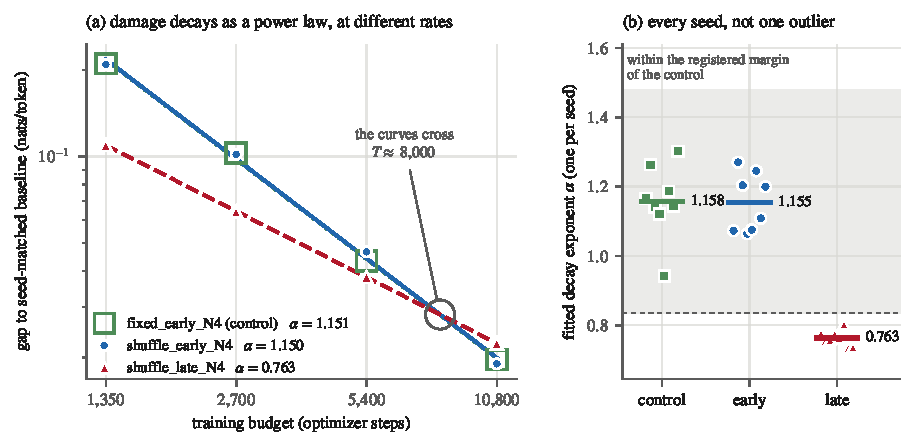
\includegraphics[width=\textwidth]{../figures/decay-v5.pdf}
\caption{Both panels are produced from the registered records; no value is
entered by hand. \textbf{(a)} On log axes a power law is a straight line and
$\alpha$ is its slope. The fitted early and late curves meet at $T \approx 7{,}987$
---inside the ladder, between the third and fourth rungs. A level endpoint would
have reported whichever side of that crossing its single budget happened to fall
on. \textbf{(b)} The late arm's eight seeds span $0.735$--$0.803$, a band
narrower than its distance from the other sixteen, so the contrast is not one
seed's doing. The control's own spread---$0.942$--$1.302$, the widest of the
three---is what the registered margin is three times of.}
\label{fig:decay}
\end{figure*}

\section{Results}

\subsection{The curves cross}

Table~\ref{tab:gaps} gives the mean gap to baseline in nats per token. Read the
first and last columns together: early damage begins nearly twice as large as
late damage and ends smaller. Figure~\ref{fig:decay} shows the same data with the
fitted power laws.

\begin{table}[t]
\centering\small
\begin{tabular}{lrrrr}
\toprule
Condition & 1{,}350 & 2{,}700 & 5{,}400 & 10{,}800 \\
\midrule
control (F, early) & .2106 & .1030 & .0434 & .0197 \\
shuffle, early     & .2091 & .1019 & .0467 & .0190 \\
shuffle, late      & .1097 & .0643 & .0381 & .0224 \\
\bottomrule
\end{tabular}
\caption{Mean gap to a seed-matched baseline, in nats/token, for
\cond{fixed\_early\_N4}, \cond{shuffle\_early\_N4} and \cond{shuffle\_late\_N4}.
Over the 8$\times$ budget increase the early gap shrinks 11.0-fold, the control's
10.7-fold, and the late gap only 4.9-fold.}
\label{tab:gaps}
\end{table}

\subsection{Early damage matches the control}

\begin{table}[t]
\centering\small
\begin{tabular}{lccrl}
\toprule
Condition & $\alpha$ & 95\% CI & $p$ & Reading \\
\midrule
control & 1.158 & [1.07, 1.25] & --- & anchor \\
early   & 1.155 & [1.09, 1.23] & .95 & like control \\
late    & 0.763 & [0.74, 0.78] & .0002 & slower \\
\bottomrule
\end{tabular}
\caption{Fitted exponents read against the control.}
\label{tab:alphas}
\end{table}

Table~\ref{tab:alphas} gives the readings. Fitting amplitude as well as exponent
sharpens this: the control and the early arm are the same power law in
\emph{both} parameters ($\alpha$ 1.151 and 1.150, amplitude 871.0 and 871.0 on
rung-mean gaps). The late arm differs in both.

\subsection{The primary contrast}

$\alpha(\text{early}) - \alpha(\text{late}) = +0.392$, two-sided exact
permutation $p = 0.0002$, against a registered margin of $0.323$. One-sided $p$
in the critical-period direction: $1.0000$.

\textbf{Registered verdict: \cond{REVERSE\_ONSET\_EFFECT}.} Onset changes the
repair rate, and the later onset is the one repaired more slowly---the reverse of
the direction this study registered in advance. The name labels that measured
relation between two exponents. It is \textbf{not} a claim that the vision
literature is contradicted; Section~\ref{sec:related} says why that comparison is
not available.

\subsection{The other registered result}

An earlier registered run, under a design differing from this one only in its
instrument, returned \cond{INCONCLUSIVE} (Table~\ref{tab:v4v5}).

\begin{table}[t]
\centering\small
\begin{tabular}{lccccl}
\toprule
Run & Seeds & Rungs & $\Delta\alpha$ & Margin & Verdict \\
\midrule
v4 & 5 & 3 & $+.438$ & .501 & \cond{INCONCL.} \\
v5 & 8 & 4 & $+.392$ & .323 & \cond{REV\_ONSET} \\
\bottomrule
\end{tabular}
\caption{Both two-sided $p$-values sit exactly on the floor of their own
permutation test ($2/252$ at five seeds, $2/12870$ at eight); the floors differ
only because the seed counts do.}
\label{tab:v4v5}
\end{table}

The effect estimate replicated; the margin did not hold. The margin is three
times the control's own per-seed scatter, and in v4 one seed's exponent came out
at 1.505 against 1.075--1.247 for the other four, because that seed's baseline at
the top rung was the worst of the five and compressed its gap. One seed roughly
doubled the margin.

The defect is direction-neutral and would have been true whichever way the effect
ran: a scale estimated from five numbers scatters by $\pm34\%$ of the truth, so
the margin can halve or double from luck alone. It did---$0.298$ on one seed set,
$0.501$ on the next.

\textbf{v5 changed the instrument and not the judgment.} The decision module
hashes identically in both freeze manifests. What changed was a fourth rung
placed \emph{below} the others---at the top rung the gap is only about eight times
the baseline seed SD, so extending upward would push further into noise---and
eight seeds instead of five.

\subsection{Robustness}

\textbf{Specification multiverse.} 144 defensible specifications: four sources for
the margin's scale $\times$ three multiples $\times$ three floors $\times$ two
exponent estimators $\times$ two rung sets, with the verdict logic held fixed.
v5's verdict holds in 138/144 (96\%), dissenting only at the widest margin taken
from the noisiest scale source. v4's holds in 90/144 (62\%)---\textbf{more than a
third of reasonable analysts would have called it positive.} Four specifications
are excluded by name with reasons rather than swept in, including anchoring on the
refuted theoretical value; including options already known to be wrong lets bad
pipelines vote.

\textbf{The recovery-asymmetry objection.} The late arm's deficit ends later, so
it has less training left: 75\% of the early arm's post-deficit steps and 51\% of
its learning-rate area. Under a level endpoint this was a genuine confound. Under
an exponent endpoint it cannot be one, because a handicap that is the same
multiple at every rung moves the amplitude and leaves the exponent exactly
unchanged---verified numerically at multipliers from 0.5 to 10, shift
$0.00\mathrm{e}{+}00$ throughout. The handicap is constant: the step ratio varies
by $0.0004$ across the ladder and the learning-rate-area ratio by $0.0009$.
Producing the observed exponent difference would require the handicap to grow as
$T^{0.387}$---2.24$\times$ more severe at the top rung than the bottom. Measured
growth: 0.18\%.

\section{What this does not show}
\label{sec:notshow}

\textbf{Whether the damage is permanent.} Answering that requires the deficit's
cost in effective training steps held constant across rungs---a pure lag is
exactly that quantity being constant---which means inverting the baseline curve.
Four rungs cannot pin it down; our exploratory attempt returned 1370, 693, 882
effective steps for the control, a non-monotonicity that is an artefact of
interpolating between too few points. The question is \textbf{dropped, not
answered}, and no exponent reported here may be pressed into service for it.

\textbf{The shape of the onset curve.} We have two onsets. Two points establish a
difference and cannot establish a shape, and the shape is not a detail: the onset
curve in \citet{achille2019critical} is non-monotonic, peaking around a tenth of
the way into their run rather than at its start. Nothing here says whether the
function relating onset to repair rate is monotonic, single-peaked, or something
else.

\textbf{A mechanism.} None is identified and none is claimed. The one
representational measure the design registered---layerwise CKA
\citep{kornblith2019similarity}---was never produced: no checkpoints were saved,
so it is not computable from the records, and re-running with checkpointing would
be a new study. We state this rather than let the registered list imply a measure
was taken.

\textbf{Anything about scale, schedule, or other deficits.} 7.34M parameters, one
corpus, one learning-rate schedule, one deficit pair, one late onset chosen by
fiat at half the clean budget.

\textbf{Anything about development or cognition.} The claim register has forbidden
any developmental reading since before data existed.

\section{Related work}
\label{sec:related}

\textbf{Vision.} \citet{achille2019critical} established the phenomenon and the
protocol, including the requirement for a control that leaves low-level
statistics intact; \citet{kleinman2024critical} show it in deep linear networks.
Their proposed mechanism---a loss of ``Information Plasticity'' read off the
Fisher Information of the weights---is a claim we neither use nor test.

\textbf{Our result is not a contradiction of that literature, and we want to be
exact about why.} \citet{achille2019critical} slide a fixed-length deficit window
across onsets and report, verbatim, that sensitivity ``peaks in the central part
of the early rapid learning phase (at around 30 epochs), while introducing the
deficit later produces little or no effect.'' Their onset curve is therefore
\textbf{non-monotonic, and a deficit at the very start of training is not its most
damaging case}. Two things follow. First, our two onsets cannot be placed on that
curve: doing so needs a normalisation between a 300-epoch CIFAR schedule and a
budget ladder from 1{,}350 to 10{,}800 steps, and none is established. Second and
more fundamentally, the two studies do not measure the same quantity. Their
sensitivity is a level---final accuracy after a fixed amount of further
training---and Section~1.1 argues that a level at one training length cannot
separate damage that is permanent from damage that is merely behind. \textbf{A
result cannot contradict a measurement that it also argues is not measuring the
thing.}

\textbf{Language models.} \citet{constantinescu2025investigating} found no
critical period for delayed second-language exposure. Ours is a second negative in
a different paradigm---degraded input during a window rather than delayed exposure
to new material---and adds a positive onset finding their design could not have
seen, since varying age of exposure does not produce a window of degraded input to
time.

\textbf{Data order and the schedule.} \citet{luo2025learning} find that
curriculum-based pretraining beats random shuffling under a constant learning rate
and loses that advantage under standard decay, concluding that data curricula must
be co-designed with the optimizer. Their setting is data quality rather than a
deficit window, but the structural point is ours: where something sits in the data
order and where it sits on the learning-rate schedule are not separable unless a
design separates them. Ours does not.

\section{Discussion}

The finding we did not expect is not the absence of a critical period---the prior
for that was already unfavourable---but the presence of an onset effect running
against the registered direction, and the precision with which early damage
matches the control. To three decimal places in the exponent and four significant
figures in the amplitude, a deficit that destroys word order at the very start of
training is repaired exactly as fast as one that merely hides it behind a fixed
code.

One reading suggests itself, and rather than leave it as a gloss that no result
could contradict, we state what would refute it. Suppose that at the very start
there is little structure to disrupt, so the corruption is paid for in training
time and nothing else. Then the early arm should be equivalent to a clean run
given a shorter budget---its damage describable as a \emph{constant} debt in
effective training steps at every rung---and the late arm should not be. That is a
prediction about exactly the quantity Section~\ref{sec:notshow} puts out of scope,
and out of scope for the same reason it is the right test. On a denser ladder,
\textbf{the early arm's debt should be flat across budgets and the late arm's
should grow.} If both are flat, or both grow, this reading is wrong.
\textbf{We have no evidence for it now.}

The methodological story may be the more transferable one. Three endpoints were
tried and discarded before this one, and each failed the same way: it smuggled a
parameter in from outside the experiment. A level at one budget smuggled in where
the run stopped. A categorical ladder verdict smuggled in an arbitrary 0.01-nat
floor. An exponent read against $\alpha = 1$ smuggled in a constant learning-curve
slope that the same data showed falling. A control-anchored comparison smuggles in
nothing: every quantity it uses is measured in the same runs.

And one procedural rule earned its place outright. \textbf{The registered run may
not reuse any seed the calibration used.} Calibration used one seed set, the first
registered run a second, the third a third. Had the first reused the calibration
seeds it would have returned \cond{REVERSE\_ONSET\_EFFECT} and the freeze would
have certified a result that a genuine out-of-sample replication does not support.
That interception is the single most valuable thing the preregistration produced.

\section{Registration and provenance}

The design was frozen before each registered run and carried by an annotated
tag;\footnote{Preregistration, claim register, frozen decision code, freeze
manifests, all 188 registered run records, the deviation log and the scripts that
regenerate every number and figure in this paper:
\url{https://anonymous.4open.science/r/ANONYMIZED} (anonymized for review).}
six files are hashed into a manifest that a check verifies, and the judgment code
is byte-identical between the two registered designs. Before the decision code was
allowed to see a real run it had to return each of its five verdicts correctly
against fabricated ladders with planted decay exponents.

\textbf{One disclosure the result must travel with.} The
\cond{REVERSE\_ONSET\_EFFECT} verdict category was added to the claim register
\emph{after} exploratory data pointed at the pattern. The exploratory data
motivated giving it a name; it supplied no evidence for it, and the registered runs
are what do. Without a name for it the design would have absorbed the most
interesting thing in its own data into a null---but the ordering is recorded so a
reader can discount it as they see fit.

Every departure from the registered design, including one attempt to annotate the
frozen text that the freeze check rejected, is in an append-only log with its date,
its reason, and whether it was decided before or after the affected result was
visible.

\section*{Limitations}

The $t$-interval on $\alpha$ is a normality assumption at eight seeds; the primary
contrast is an exact permutation test and does not depend on it. The power law is
fitted over an 8$\times$ budget range and is an extrapolation outside it.

The late onset is fixed at half the clean budget by fiat, and there are only two
onsets, so the shape of the onset curve is not identified.

\textbf{Onset and learning-rate position are confounded by construction.} Moving
the deficit window moves it along the cosine schedule at the same time, so ``when
in training'' and ``at what learning rate'' cannot be separated here.
\citet{pawlak2025occurence} reports that restarting the rate undoes
critical-period damage in vision, which is direct evidence that schedule position
does work in this class of effect. Separating the two needs a design that holds one
fixed while moving the other.

Top-rung precision limits everything: the gap there is about eight times the
baseline seed SD, and log-space fitting turns top-rung noise into exponent noise.
This is what produced the v4 outlier and, through the margin, the v4 verdict.

Three pilots failed before the first valid ladder---a wrong denominator, a refuted
control, a warmup that did not scale---for reasons no amount of simulation would
have found.

Everything here is one model size on one corpus. Nothing in this paper licenses a
claim about production-scale pretraining.

\bibliography{custom}

\end{document}
